\chapter{Linear Cross Entropy in the Projective Transverse-Field Ising Model}
\label{ch:lxe-ptim}
For now, this chapter serves to test the limits of this layout, i.e. have a
ridiculously long chapter name, an epigraph with citation, sections,
subsections, subsubsections, paragraphs, itemizes, descriptions, \ldots
I will possibly also test the math mode here, but that is probably just a font
issue.
\section{The Beginning!}
First of all, let's cross-reference a whole lot of stuff: \cref{ch:intro} and
\cref{ch:basics} as well as \cref{fig:firstattempt-lxe}

\begin{figure}
  \centering
  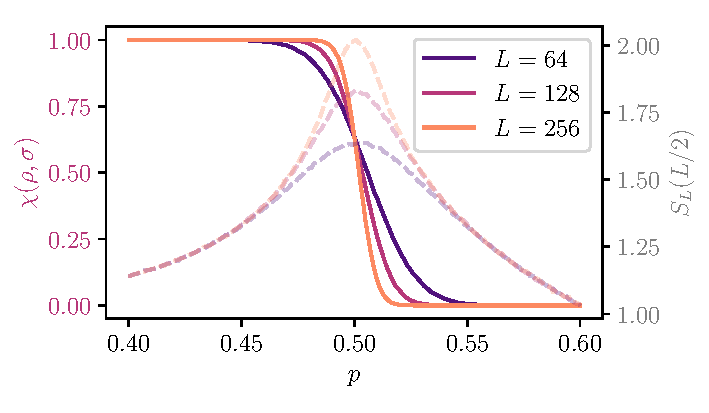
\includegraphics{simple_lxe_ptim_three_sizes_circuits.pdf}
  \caption{Let's see if the colormap synergizes with the rest of the layout. I
  sure do hope so.}
  \label{fig:firstattempt-lxe}
\end{figure}

\lipsum[0-2]
Nielsen \cite{nielsenQuantumComputationQuantum2010} Gottesman
\cite{gottesmanStabilizerCodesQuantum1997}
\cite{aaronsonImprovedSimulationStabilizer2004}
\section{WOAH!}
\lipsum[3]
entropy in stabilizer formalism
\cite{fattalEntanglementStabilizerFormalism2004}
ptim nicolai \cite{langEntanglementTransitionProjective2020}
\subsection{Coole Subsection}
\lipsum[4-6]
\cite{roserDecodingProjectiveTransverse2023}
\subsubsection{Coole Subsubsection}
\lipsum[7-9]
\subsubsection{Dies ist ein Test!}
\lipsum[10-11]
\subsection{Noch ein Test!}
\lipsum[12-14]
\cite{tikhanovskayaUniversalityCrossEntropy2023}
\section{Neue Section mit mehreren Equations aus der BA}
Diese Section ist geklaut aus meiner BA. Da dort ein paar wilde Mathesachen
vorkommen, dachte ich dass es vielleicht ein guter Test ist sowohl für Layout
als auch Typeface.

In classical Hamiltonian mechanics the state of a system (at some time $t$) is
represented by a point $\xi$ in phase space, which, for a system with $n$
degrees of freedom, resides in $\mathbb{R}^{2n}$
\cite{noltingHamiltonMechanik2014}.\\
According to the first postulate of quantum mechanics, the state of a system
(at time $t$) is defined by a unit vector in Hilbert space $\mathcal{H}$,
called \emph{state vector} \cite{cohen-tannoudjiQuantumMechanicsVolume1977}.
This gives rise to an
intriguing fundamental difference to the classical world, since any arbitrary
vector (in $\mathcal{H}$) can be represented as a linear combination of basis
vectors.  This is called the superposition principle
\cite{poschelFourierreihen2015, messiahQuantumMechanics1991}.
Let us consider the fundamental example of a two-state system, with a ground state '0' and an excited state '1'.
Note that in the context of quantum information this type of system is referred to as \emph{qubit}.
The most general state of the system is described by a superposition of the two states,  
\begin{align}\label{eq:superpos}
    \ket{\psi} = c_1 \ket{0} + c_2 \ket{1}.
\end{align}
In \cref{eq:superpos}, quantum states are represented using the so-called Bra-Ket-notation. 
The state vector of a quantum system in $\mathcal{H}$ is denoted by $\ket{\psi}$\footnote{read: Ket $\psi$. Also called \emph{Ket-vector}},
with the corresponding vector $\bra{\psi}$\footnote{read: Bra $\psi$. Also called \emph{Bra-Vector}} in dual space.
The inner product on $\mathcal{H}$ is then defined as
$\braket{\varphi}{\psi}$.
\par
Since states are elements of a complex vector space, they are not physical observable quantities. Therefore, the formalism
has to be complemented with a mathematical formalism of observables in order to get a complete and meaningful description of quantum systems.
In general, physical quantities can be measured (observed) and the outcome of such a measurement should therefore be
a real\footnote{as opposed to complex} number.
For this we employ the second postulate of quantum mechanics. It states that measureable physical quantities
(observables) are Hermitian operators acting in $\mathcal{H}$. 
The Hermitian property implies that the operator only has real eigenvalues, is diagonalizable,
and that its eigenvectors are orthogonal \cite{messiahQuantumMechanics1991}.\\
%We measure by applying an operator of an observable $\hat{A}$ to the state vector $\ket{\psi(t)}$ is called measuring.
Let us convince ourselves of the advantages that come with this Hermitian property.
Suppose we want to measure some observable $A$.
The outcome of such a measurement is an eigenvalue $a_k$ of the operator $\hat{A}$. The probability to observe the specific outcome $a_k$ is
\begin{align}\label{eq:prob-meas}
    p(a_k) = \braket{\psi}{a_k}\braket{a_k}{\psi} = \abs{\braket{a_k}{\psi}}^2,
\end{align}
where $\bra{a_k}$ are the eigen-bras of $\hat{A}$ with eigenvalue $a_k$.\\
Due to the inherent probabilistic description of quantum mechanics (cf. \cref{eq:prob-meas}), we can only make meaningful statements about averages.
Weighing every eigenvalue $a_k$ with its respective probability to be measured
given by \cref{eq:prob-meas}, the average of an observable becomes
\cite{nielsenQuantumComputationQuantum2010}
\begin{align}
    \expval{\hat{A}} = \sum\limits_k a_k p(a_k) = \sum\limits_k a_k \braket{\psi}{a_k}\braket{a_k}{\psi}
    = \bra{\psi} \left(\sum\limits_k a_k \dyad{a_k}\right) \ket{\psi} = \ev{\hat{A}}{\psi}.
\end{align}\\
Let us consider a concrete example of an operator.
Arguably the most essential operator in quantum mechanics is the Hamilton operator $\hat{H}$, often simply abbreviated as Hamiltonian.
It describes the total energy of a system, and is the generator of time translation, i.e. time evolution. A state vector evolves
according to the \emph{Schrödinger equation}, defined as
\cite{messiahQuantumMechanics1991}
\begin{align}\label{eq:schro-eq}
    i\partial_t \ket{\psi(t)} = \hat{H} \ket{\psi(t)}.
\end{align}
Solving \cref{eq:schro-eq} gives us
\begin{align}\label{eq:schro-sol}
    \ket{\psi(t)} = e^{-i\hat{H}t}\ket{\psi(0)} \equiv U(t)\ket{\psi(0)}
\end{align}
with $U(t)$ defined as the unitary time evolution operator. Unitary operators fulfil the relation $UU^\dagger=\mathds{1}$, i.e.
its inverse is given by its Hermitian conjugate. Using the fact that the Hamiltonian is a Hermitian operator, unitarity follows from 
\begin{align}\label{eq:unitary-property}
    U(t)U^\dagger(t) = e^{-i\hat{H}t}e^{i\hat{H}^\dagger t} = e^{-i\hat{H}t}e^{i\hat{H}t} = \mathds{1}.
\end{align}
The determinant of such an operator is $1$, meaning that
the state vector the operator acts upon keeps unit length during its time evolution.
\par
In \cref{eq:schro-sol} and \cref{eq:unitary-property} we used the exponential of an operator. Since the
product of operators and
the series expansion of the exponential function are well defined, the exponential of an operator is defined through series expansion.
For instance, the series expansion of $U(t)$ becomes
\begin{align}\label{eq:matrix-exp}
    U(t) = \sum\limits_{n=0}^\infty \frac{(-i\hat{H}t)^n}{n!}.
\end{align}

